\documentclass[dvipdfmx]{jarticle}
\pagestyle{empty}
\usepackage{tikz}
\usetikzlibrary{shapes,calc}
\begin{document}
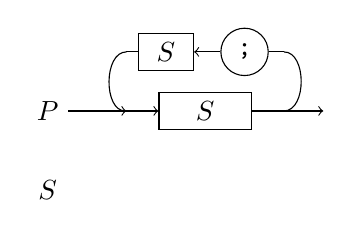
\begin{tikzpicture}
  \node (P0) at (0,0) {$P$};
  \node[draw] (P1) at ($(P0)+(2,0)$) {\mbox{\quad $S$\quad }};
  \node[draw,circle] (P2) at ($(P1)+(0.5,0.75)$) {\texttt{;}};
  \node[draw,rectangle] (P3) at ($(P1)+(-0.5,0.75)$) {\mbox{\ $S$\ }};
  \path[->] (P0) edge (P1);
  \path[->] (P1) edge ($(P1)+(1.5,0)$);
  \path[-] ($(P1)+(1,0)$) [out=0,in=0] edge ($(P1)+(1,0.75)$);
  \path[-] ($(P1)+(1,0.75)$) edge (P2);
  \path[->] (P2) edge (P3);
  \path[-] (P3) edge ($(P3)+(-0.5,0)$);
  \path[->] ($(P3)+(-0.5,0)$) [out=180,in=180] edge ($(P1)+(-1,0)$);
  \node (S0) at (0,-1) {$S$};
\end{tikzpicture}
\end{document}